% 
% ======================================================================
\RequirePackage{docswitch}
% \flag is set by the user, through the makefile:
%    make note
%    make apj
% etc.
\setjournal{\flag}

\documentclass[\docopts]{\docclass}

% You could also define the document class directly
%\documentclass[]{emulateapj}

% Custom commands from LSST DESC, see texmf/styles/lsstdesc_macros.sty
\usepackage{lsstdesc_macros}

\usepackage{graphicx}
\graphicspath{{./}{./figures/}}
\bibliographystyle{apj}
% Add your own macros here:


% 
% ======================================================================

\begin{document}

\title{ Inference of the Conditional Luminosity Function by Explicit Marginalization over All Individual Galaxy Parameters }

\maketitlepre

\begin{abstract}

We explore a hierarchical model for galaxy luminosities and halo masses whose hyperparameters govern the conditional luminosity function, and whose many individual object parameters are explicitly marginalized over. 
We investigate four techniques to perform the high dimensional marginalization, and comment on their performance. 

\end{abstract}

% Keywords are ignored in the LSST DESC Note style:
\dockeys{Galaxies: halos, Galaxies: statistics, Methods: numerical}

\maketitlepost

% ----------------------------------------------------------------------
%

\section{Introduction}
\label{sec:intro}

The large scale structure of the universe is dominated by the collective gravitational influence of dark matter particles and the repulsive force of dark energy.
There are ongoing efforts to infer the masses and locations of dark matter halos and improve measurements of dark energy parameters.
Observational progress has been gradual, creating opportunity for simulations.
Given a cosmology, large N-body simulations can predict characteristics like clustering and the halo mass function with high precision \citep*[eg.][]{nbody}.
Simulated universes are readily available and inspire our effort to connect theory to empirical observations.

The halo mass and galaxy luminosity relation is a conduit between dark matter halos and galaxy observations. 
The conditional probability allows us to convert the dark matter halos from simulations into distributions of galaxy luminosities in different redshift bins that we can compare with observations.
The exact form of the relation is an active area of research; models that separate central and satellite galaxies have been proposed \citep[eg.][]{satellites}.

Weak lensing is another technique that can characterize the halo composition of our universe. 
The gravitational influence of a massive dark matter halo causes the light from nearby galaxies to bend as it passes by, leading to a shearing effect. 
Over a swathe of sky, typically on the order of 1000s of square arcminutes, the collective shears allow the masses and locations of halos to be weakly inferred. 
These inferences grow stronger as the density of galaxy observations increases.
The ongoing Dark Energy Survey and upcoming Large Synoptic Survey Telescope will provide dense galaxy catalogs which will increase the potential of this approach \citep{des, lsst}. 

Traditionally the mass luminosity relation and weak lensing have been pursued in isolation, each ignoring information the other could provide. 
It is our goal to harness the full constraining power of observations by modelling both weak lensing and the mass luminosity relation in a self consistent, heirarchical framework.
We employ the mass luminosity relation described in \citet{reddick} and the mass mapping infrastructure from 
\citet{components}. 
Figure \ref{fig:ultimate_pgm} outlines the dependencies of our ultimate model.

\begin{figure}[h]
\centering
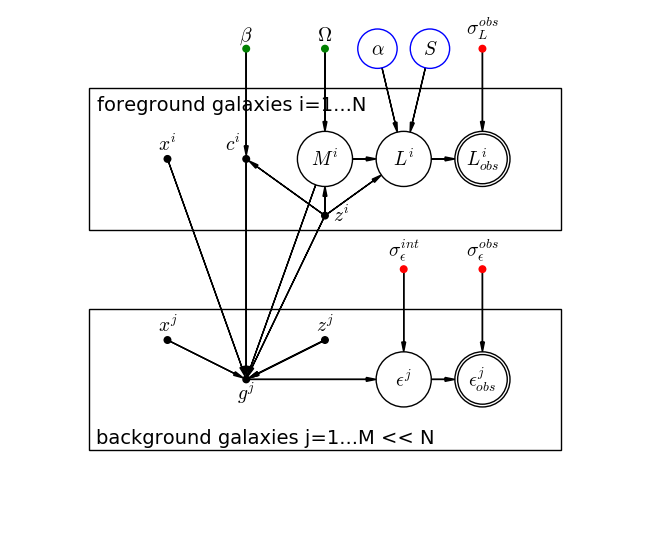
\includegraphics[width=0.9\columnwidth]{ultimate_pgm.png}
\caption{
A probabilistic graphical model for the model we ultimately aspire to. 
There are two plates; one for foreground galaxies, one for background galaxies. 
The cosmology hyperparameters are colored green, the mass luminosity relation hyperparameters are colored blue, and the noise hyperparameters are colored red. 
$\beta$ represents the form of the halo concentration.
$\Omega$ represents the cosmology used to generate the halos in the Millennium Simulation.
$\alpha$ represents four parameters that convert mass to mean luminosity, and $S$ represents the scatter of the corresponding lognormal.
$M,L$ represent mass and luminosity respectively. 
The variables $x,z$ denote angular position and redshift respectively.
$c$ is for the concentration, $g$ is for the reduced shear, and $\epsilon$ is for the shear.
Finally, $\sigma$ represents various forms of noise and the superscript \emph{obs} is used to denote an observational noise or observable. 
\label{fig:ultimate_pgm}}
\end{figure}

The model partitions galaxies into two groups. 
Background galaxies are sources that lie in a redshift bin immediately behind the three dimensional space of foreground galaxies. 
The background galaxies provide the observed shears which we use to infer the halo masses of foreground galaxies. 
We plan to use around 200,000 foreground galaxies and 1,600 background galaxies in our model and analysis. 
In the course of the heirarchical inference, each of the 200,000 galaxies contributes and has a corresponding mass and luminosity which must be marginalized out. 
Given the large size of our inference, we expect the primary challenges to be computational in nature - how can we achieve inference at this unprecedent scale?
In order for us to rapidly iterate towards an answer to this question, we study a model with simpler dependencies.
This condensed model, shown in Figure \ref{fig:simplified_pgm}, offers the benefit of being easier to test while retaining the computational challenges that need to be adressed.

\begin{figure}[h]
\centering
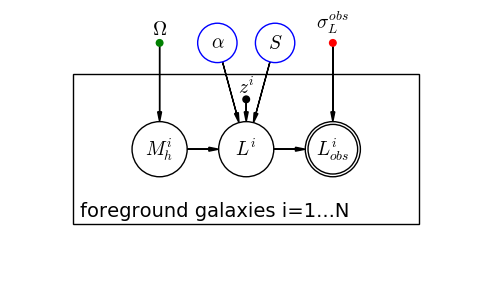
\includegraphics[width=0.9\columnwidth]{simplified_pgm.png}
\caption{
A probabilistic graphical model for the simplified model we will use for testing.
The parameters are a subset of those in Figure \ref{fig:ultimate_pgm}.
\label{fig:simplified_pgm}}
\end{figure}

The data we use is derived from the Millennium Simulation \citep{millennium}. 
Our selection is driven by our desire to incorporate weak lensing into our ultimate model, which necessitates the large number of halos. 
Furthermore, \citet{raytracing} have also performed raytracing on this dataset which we plan to make use of in our weak lensing inference. 
There are two transformations that are applied on top of the simulation output.
First, a friend-of-friend (FoF) group finding algorithm identifies halos from the particle concentrations in the simulation output. Second, a $40 \times 40$ square arcminute window of sky out to redshift 3.5 is carved out from the output. 
The interior halos form the foreground galaxies in our analysis.  
The resulting dataset consists of 115,919 halos with accompanying positions (right-ascension, declination, and redshift).

The statistical inference we perform follows the canonical inference formula: posterior equals prior times likelihood. 
In the analysis that follows we use an overline, such as $\overline{z}$, to distinguish a vector over all foreground galaxies from the variable corresponding to a single halo, or $z$.
Given the mass luminosity hyperparameters $\alpha$, $S$; a vector of observed luminosities $\overline{L^{obs}}$; a vector of redshifts $\overline{z}$; and the observational noise in luminosity measurements $\sigma_L^{obs}$ - the posterior we seek is
$$\underbrace{P(\alpha, S| \overline{L^{obs}}, \overline{z}, \sigma_L^{obs})}_{
	\text{Posterior}} = 
\underbrace{P(\alpha, S)}_{\text{Prior}} \underbrace{P(\overline{L^{obs}}| \alpha, S, \overline{z}, \sigma_L^{obs})}_{\text{Likelihood}}$$

Using the probabilistic graphical model we can further factor this to

\begin{align*}P(\alpha, S| \overline{L^{obs}}, \overline{z}, \sigma_L^{obs}) &= P(\alpha)P(S) \\
 \iint \overline{dM}\ \overline{dL}\ &P(\overline{L^{obs}}| L, \sigma_L^{obs}) P(\overline{L}|\overline{M},\alpha,S,\overline{z})P(\overline{M}|\overline{z})
\end{align*}

The likelihood integral involves integrating over 200,000 variables - the mass and luminosity for each galaxy in our dataset. 
The Methods section of this paper describes various approaches to make such a high dimensional integral computationally tractable. 

The integrand of the likelihood contains three probabilities. 
The first is the conditional observed luminosity probability. 
Since luminosities are usually reporeted in log-space, we assume that there are gaussian errors in the log-space luminosity measurements, or that the distribution is log-normal. 
We believe 5\% errors seem reasonable and fix $\sigma_L^{obs} = 0.05$. Our conditional distribution is 

$$P(\overline{L^{obs}}| \overline{L}, \sigma_L^{obs}) = \frac{1}{\overline{L^{obs}}\sigma_L^{obs}\sqrt{2\pi}}\exp\left(-\frac{(\ln \overline{L^{obs}} - \ln \overline{L})^2}{2\sigma_L^{obs\ 2}}\right)$$

The second factor in the likelihood integrand is the mass luminosity relation $P(\overline{L}|\overline{M},\alpha,S,\overline{z})$. 
We use the form described in \cite{reddick}. 
Reddick follows the convention from previous work where the conditional luminosities is divided into two parts, central and satellite galaxy contributions. 
The central contribution is described by a lognormal distribution and the satellite contribution is described by a Schechter function. 
In our analysis, we ignore the satellite contribution. 
This decision is made for convenience, and we can easily insert the satellite contribution in future analyses. 
We use $\alpha = (\alpha_1, \alpha_2, \alpha_3, \alpha_4)$ to represent the parameters for computing the mean luminosity and $S$ for the scatter. 
This gives

\begin{align*}
P(\overline{L}|\overline{M},\alpha,S,\overline{z}) &= \frac{1}{\overline{L}S\sqrt{2\pi}}\exp\left(-\frac{(\ln \overline{L} - \ln \overline{\mu_L})^2}{2S^{2}}\right)\\
\mu_L &= \exp(\alpha_1) \cdot \left(\frac{M}{\alpha_3}\right)^{\alpha_2} \cdot (1+z)^{\alpha_4}\\
\end{align*}

The third factor in the likelihood integrand is the halo mass function $P(\overline{M}|\overline{z})$. 
For this we rely on the python software package \emph{hmfcalc} \citep*{hmf}. 
In the API we select the functional form from \citep{tinker} and the cosmology from the Millennium Simulation to govern the mass function. 
The API returns 400 logarithmically spaced mass samples and the derivative of the number density $\frac{dn}{dM}$. 
We convert this into a probability density with trapezoidal integration.
The function also has a dependence on redshift, which we account for by employing 20 redshift bins and matching the halos in the different redshift bins with the corresponding prior.
Figure \ref{fig:priors} shows the priors for each redshift bin.

\begin{figure}[h]
\centering
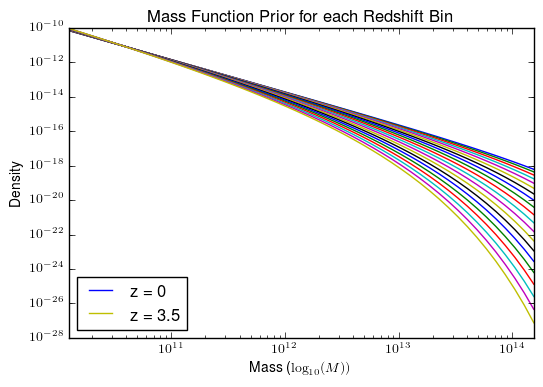
\includegraphics[width=0.9\columnwidth]{priors.png}
\caption{
The mass function prior for the range of redshift bins from z = 0 to z = 3.5.
\label{fig:priors}}
\end{figure}

In Subsection \ref{subsec:epsilon_back} we discuss further modifications to the prior that allow it to work in concert with both sampling and logarithms. 


% ----------------------------------------------------------------------

\section{Methods}
\label{sec:methods}

The primary challenge this paper seeks to resolve is computing the high dimensional likelihood integral.
In order to experiment with different methods and measure their performance, we develop a standardized benchmark in the form of a synthetic dataset.
Then we describe four different likelihood integration approaches. 

\subsection{Test Dataset}
\label{subsec:testdata}

The hyper-parameters of our model are $\alpha_1, \alpha_2, \alpha_3, \alpha_4, S$ - which govern the conditional luminosity relation describe in Section \ref{sec:intro}.
Our test dataset is generated by taking a random sample of these hyper-parameters from the distributions suggested in \citet{reddick}, the draw is shown in Figure \ref{fig:drawn}.
Starting with the halos - and their corresponding masses and positions - in our original dataset we use the drawn hyper-parameters to generate luminosities and observed luminosities.
Then we can validate our proposed methods for computing the likelihood by checking whether the corresponding posteriors are maximized at the point in hyper-parameter space that we generated the data with. 

\begin{figure}[h]
\centering
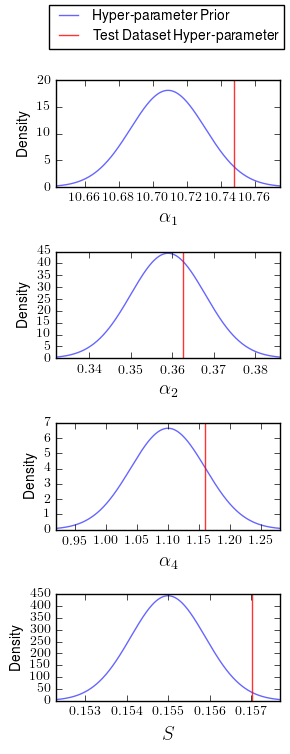
\includegraphics[width=0.9\columnwidth]{drawn.png}
\caption{
The hyper-parameter distribution is shown in blue and the drawn hyper-parameter value for the test dataset is shown in red.
\label{fig:drawn}}
\end{figure}


The original likelihood integral can be factored into a product of integrals corresponding to each halo. 
Letting $D$ be the dataset of halos we have

\begin{align*}
\mathcal{L}(L^{obs}|\alpha, S, \sigma_L^{obs}, z) = \prod_{(L^{obs}, z) \in \text{D}} &\\
\left(\int dM\ dL\ P(L^{obs}| L, \sigma_L^{obs})P(L|M,\alpha,S,z)P(M|z)\right) &\\
\end{align*}

Initially, we narrow our focus to a single one of these integrals. 
After we characterize the tradeoffs in the single integral case we expand our analysis to computations of the entire product of integrals. 

\subsection{Numerical Integration}
\label{subsec:numint}

Numerical integration is the canonical way to approximate a continuous integral on a computer.
The domain of integration is partitioned into small rectangles.
Then the integrand is evaluated at the center of each rectangle and multiplied by the surrounding rectangle's area to approximate.
This approximates the true region under the curve over the rectangle.
Summing up the contributions from all the rectangles in the domain provides an approximation of the entire integral.

The precision can be sensitive to the partitioning of the domain. 
Smaller rectangles around a point will provide more precise approximations. 
By increasing the number of rectangles in the partition, and decreasing their area, one can expect to achieve a more precise approximation of the integral.
The partitioning in the mass dimension is somewhat limited by our prior, which is comprised of a normalized, linear approximation on the 410 mass values provided by \emph{hmfcalc}. 
Breaking the mass up into more than 410 pieces would increase our reliance on the linear approximation of our prior when computing the integrand, which limits its benefit.
In our implementation we fix the mass partitioning to be the same 410 masses provided by \emph{hmfcalc}.
The runtime is $O(mn)$ where $m$ is the number of mass partitions and $n$ is the number of luminosity partitions.
In our experiments we found the scale of the luminosity partition, linear or logarithmic, to have limited impact on the result and have chosen to stick with logarithmic for slightly improved accuracy when $n$ is small. 

\begin{align*}
&\mathcal{L}(L^{obs}|\alpha, S, \sigma_L^{obs}, z) = \\
&\int dMdL\ P(L^{obs}| L, \sigma_L^{obs}) P(L|M,\alpha,S,z)P(M|z) =\\
&\sum_{M \in P_M}\sum_{L \in P_L} \Delta_M\Delta_L\ P(L^{obs}|L, \sigma_L^{obs})P(L|M, \alpha, S, z)P(M|z)\\
\end{align*}

Most of the contribution to the value of the integral comes from a small region in the domain. 
Intuition suggests that if we were able to selectively sample from this region we would be able to compute the integral more efficiently. 
This line of thought leads us to simple monte carlo integration.


\subsection{Simple Monte Carlo}
\label{subsec:smc}

Simple monte carlo integration is a method for computing an integral when the variables of integration are probabilities in the integrand.
We can approximate the integral over the probability distribution with samples from the distribution. 
In our likelihood, we employ this approximation for both the conditional luminosity $P(L|M, \alpha, S, z)$ and the prior $P(M|z)$. With these modifications our integral becomes

{\scriptsize
\begin{align*}
\mathcal{L}(L^{obs}|\alpha, S, \sigma_L^{obs},z) &= \iint dLdM P(L^{obs}|L, \sigma_L^{obs})P(L|M, \alpha, S, z)P(M|z)\\
&= \frac{1}{N_s}\sum_{M \sim\ P(M|z)}\sum_{L \sim\ P(L|M, \alpha, S, z)} P(L^{obs}|L, \sigma_L^{obs})\\
\end{align*}
}

This joint sampling generates samples with larger products $P(L|M, \alpha, S, z)P(M|z)$.
It could be that the remaining factors in the integrands, $P(L^{obs}|L, \sigma_L^{obs})$, have low weights and mitigate the benefits of this sampling.
This would happen if a halo has an outlier observed luminosity and is not sampling nearby luminosities.
Our setup is particularly prone to this because of a major disparity between our mass function prior and the masses from the dataset at the high end of the spectrum. 
This suggests that this approach may not be able to accurately compute the likelihood for halos with large observed luminosities.

\subsection{Importance Sampling}
\label{subsec:is}

Consider the large outlier observed luminosity case, where simple monte carlo is generating many low mass, low luminosity samples and poorly characterizing the integral. 
Ideally, we would be able to use the information that the known observed luminosity is large to encourage more samples in the higher mass and luminosity region.
Importance sampling is a tool that allows us to do this without biasing the result. 

The basic idea is that we multiply the integrand by $1 = Q/Q$ where $Q$ is the biased distribution we would like to sample from, and is nonzero over the domain of integration.
Then instead of sampling from our original distribution $P$, we sample from $Q$ and weigh the samples by $P/Q$.
For example, if our simple monte carlo sampling is $\int dx\ P(x) = \int dP(x)$, then the importance sampling integral is $\int dx\ \frac{P(x)Q(x)}{Q(x)} = \int dQ(x)\ \frac{P(x)}{Q(x)}$.
Appendix \ref{subsec:is_unbiased} exhibits the proof that this technique is unbiased, or that importance sampling does not change the true value of the integral.
This gives us the freedom to design our biased distribution $Q$ strategically, or so that it samples the `important' region where the weights $P/Q$ are high.

Recall that both the conditional luminosity and conditional observed luminosity relations are lognormal.
Given an observed luminosity, we can reverse the lognormal, keeping the same mean, to generate an approximate distribution of luminosities.
For example, to get $L^{obs}$ from $L$ we would take samples from the integrand factor $P(L^{obs}| L, \sigma_L^{obs})$.
To get an approximation of $L$ from $L^{obs}$ we can use 

$$Q(L|L^{obs}, \sigma_L^{obs}) = \frac{1}{L\sigma_L^{obs}\sqrt{2\pi}}\exp\left(-\frac{(\ln L - \ln L^{obs})^2}{2\sigma_L^{obs\ 2}}\right)$$

Similarly, to get an approximation of $M$ from $L$ we reverse the conditional luminosity relation, and reverse the corresponding mean mass luminosity relation as well.

\begin{align*}
Q(M|L,\alpha,S,z) &= \frac{1}{MS_Q\sqrt{2\pi}}\exp\left(-\frac{(\ln M - \ln \mu_M)^2}{2S_Q^{2}}\right)\\
\mu_M &= \alpha_3 \left(\frac{L}{\exp(\alpha_1)(1+z)^{\alpha_4}}\right)^{1/\alpha_2}\\
\end{align*}

The reader may notice how on the right hand side of the first equation above we have replaced $S$ with $S_Q$. 
This is because we use $S_Q = \lambda \cdot S$, where $\lambda$ is the constant which converts the scatter in conditional luminosity to the scatter in conditional mass.
We derive $\lambda$ through an error propagation technique in Appendix \ref{subsec:error_prop}.
Combining the above distributions into a joint biased distribution for importance sampling yields the formula below for the single halo likelihood integral.

{\fontsize{4}{5}\selectfont
\begin{align*}
&\mathcal{L}(L^{obs}|\alpha, S, \sigma_L^{obs}, z) = \\
&\iint dLdM \frac{P(L^{obs}|L, \sigma_L^{obs})P(L|M, \alpha, S, z)P(M|z)Q(L|L^{obs}, \sigma_L^{obs})Q(M|L,\alpha, S, z)}{Q(L|L^{obs}, \sigma_L^{obs})Q(M|L,\alpha, S, z)} =\\
&\frac{1}{N_s}\sum_{M \sim Q(M|L,\alpha, S, z)} \sum_{L \sim Q(L|L_{obs}, \sigma_{obs})}\frac{P(L^{obs}|L, \sigma_L^{obs})P(L|M, \alpha, S, z)P(M|z)}{Q(L|L^{obs}, \sigma_L^{obs})Q(M|L,\alpha, S, z)}\\
\end{align*}
}

To validate the effectiveness of the biased joint distributions (the Q's) we generate nine different test datasets by sampling from the priors of the hyper-parameters as described in Subsection \ref{subsec:testdata}. 
Figure \ref{fig:isworks} shows the nine corresponding scatterplots of the first 1,000 samples in the mass and luminosity dimensions. 
We see that simple monte carlo has poor coverage of the the high mass, high luminosity region as we expected.
Importance sampling on the other hand does a good job of covering the true joint distribution from the data, but is not perfect.
In the extreme upper right corner in the high mass, high luminosity region we can see places where even importance sampling is a bit off from the true distribution. 
Can we still produce a posterior distribution that is both accurate and precise?
To resolve this question we implement the integration and highlight the results in Section \ref{sec:results}.

\begin{figure}[h]
\centering
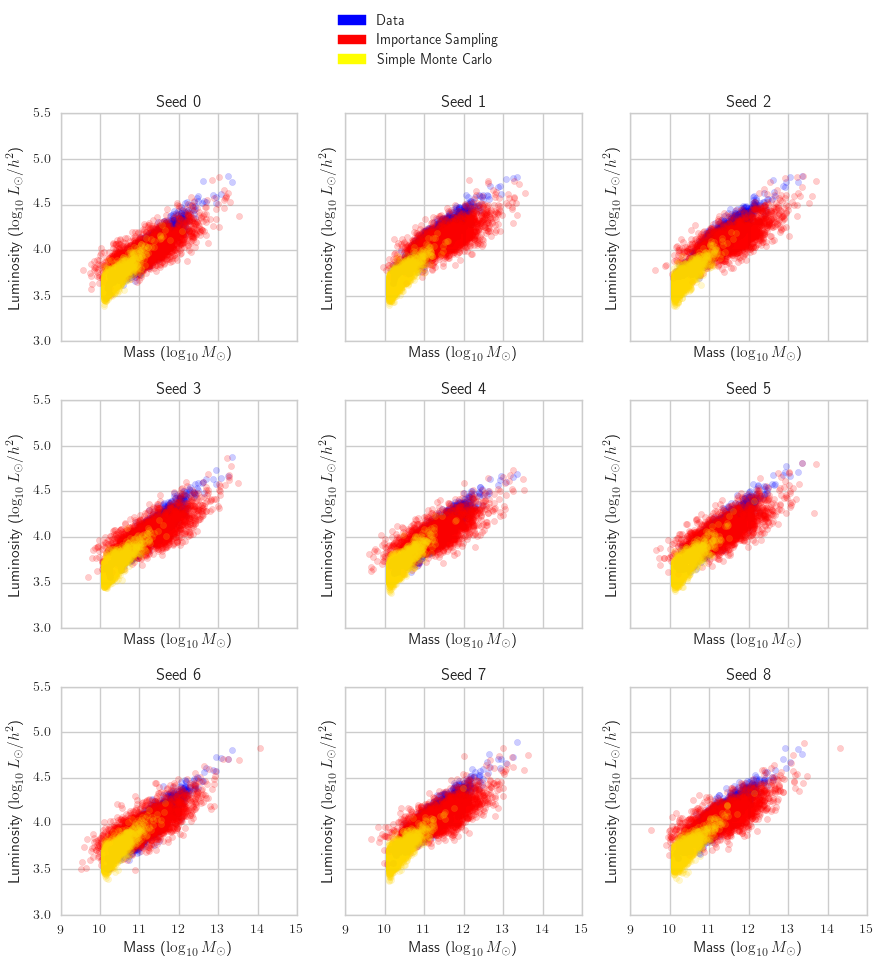
\includegraphics[width=0.9\columnwidth]{isworks.png}
\caption{
Each seed corresponds to a different draw of hyper-parameter values. The true disjoint distribution from the test dataset is in blue, the importance sampling sampling distribution is in red, and the simple monte carlo sampling distribution is in yellow.
\label{fig:isworks}}
\end{figure}

\subsection{Laplace Approximation}
\label{subsec:laplace}

The final scheme we explore adheres to paradigms from optimization. 
In this paradigm we view the integrand as a smooth surface with a hill that corresponds to the high weight, or important region of the integrand. 
To compute the integral we iteratively hike up the landscape to the highest point on the hill, the maximum of the integrand. 
From this vantage point we approximate the hill with an easy-to-integrate multivariate distribution centered on the maximum. 
The integral of the distribution serves as a rough approximation of the original integral.

To find the maximum of the integrand we use the Broyden-Fletcher-Goldfarb-Shanno (BFGS) method implemented in \emph{scipy.stats.minimize} \citep{scipy}. 
We pass the negative-log-integrand, $-\ln I(M,L)$, to the optimizer which returns the optimal point $(M^{opt}, L^{opt})$ and the inverse hessian matrix $H^{opt\ -1}$ at the optimum. 
We then approximate the integrand as 

{\tiny
\begin{align*}
I^*(M,L) = &\\
I(M^{opt}, L^{opt})\exp\left(\frac{((M,L) - (M^{opt}, L^{opt}))^TH^{opt}((M,L) - (M^{opt}, L^{opt}))}{2}\right)&\\
\end{align*}
}

\noindent which has the closed form integral 

$$\iint dMdL\ I^*(M,L) = \sqrt{\frac{4\pi^2}{\det(H^{opt})}}$$

\noindent In practice we must also apply a numerical trick to produce satisfactory inverse hessian matrices from the optimizer. Appendix \ref{subsec:rescale_la} describes this technique in detail.

% ----------------------------------------------------------------------

\section{Results}
\label{sec:results}

\subsection{Single Halo}

The likelihood integration methods discussed in Section \ref{sec:methods} can be summarized as generating sample halos, assigning them a weight, and accumulating the weights into the returned solution. 
The sampled halos and their corresponding weights serve as a good basis of comparison between methods. 
We can make this comparison more informative by extending it beyond one single likelihood of one halo to the single likelihoods of a test suite of halos. 
Each single likelihood of a halo is dependent on the halo to which it corresponds. 
To discern general patterns between methods, we make the above comparison over a test suite of halos strategically selected from the dataset.
We construct the test suite with a combination of boring, representative halos and outlier halos which we anticipate will further expose key differences. 
Figure \ref{fig:joint} shows the joint mass and luminosity distribution of the test dataset and the four points we have chosen for our test suite.
Point 2 is in the high probability region of the distribution, Point 0 is a typical point, and Point 1 and Point 3 are outliers. 

\begin{figure}[!h]
\centering
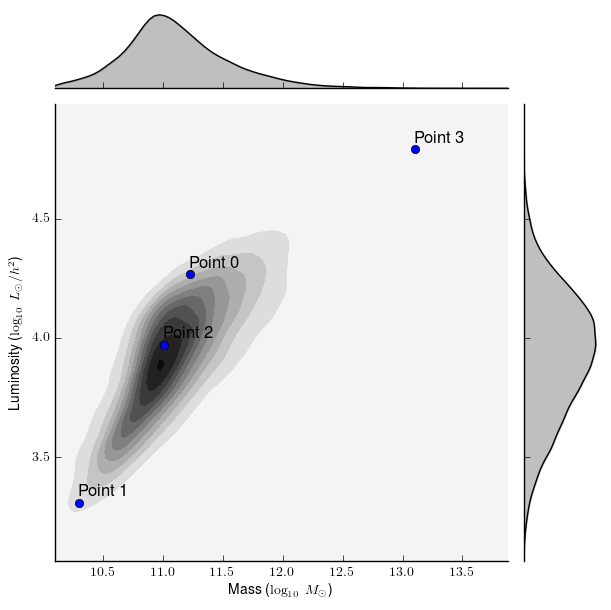
\includegraphics[width=0.9\columnwidth]{joint.png}
\caption{
The mass and luminosity joint distribution from the test dataset is shown in gray and the four points in the test suite are shown in blue. 
\label{fig:joint}}
\end{figure}

Let's step through the panel in Figure \ref{fig:point1} which corresponds to Point 0.
The plot corresponding to Numerical Integration is in the upper right.
The black dot is the true mass and luminosity of the halo whose likelihood we are computing.
The nearby black band shows the mean and standard deviation of the luminosity distribution from our test dataset, conditioned on both mass and redshift bins.
This helps us understand whether the likelihood halo is an outlier.
The points of the plot are the halos sampled by the method.
For the laplace approximation we use the optimal point after each iteration as the set of samples.
The light gray dotted line between them shows the order of the optimal path. 
The two ovals around the optimal point are the 1$\sigma$ and 2$\sigma$ epigraphs of the laplace approximation multivariate gaussian.
The color of the point shows the \emph{weight} it contributes to the likelihood.
In numerical integration and laplace approximation the weight is the original integrand $P(L^{obs}|L, \sigma_L^{obs})P(L|M, \alpha, S, z)P(M|z)$.
In simple monte carlo and importance sampling, we use the concept of \emph{weight} to distinguish from the probability density functions in the numerator that are used to generate samples from the ones that are evaluated and contribute to the sum.
In simple monte carlo the weight is $P(L^{obs}|L, \sigma_L^{obs})$ and in importance sampling the weight is $\frac{P(L^{obs}|L, \sigma_L^{obs})P(L|M, \alpha, S, z)P(M|z)}{Q(L|L^{obs}, \sigma_L^{obs})Q(M|L,\alpha, S, z)}$.
The different weight functions have different ranges.
To increase the informativeness of the panel we cap the weights for numerical integration, simple monte carlo, and importance sampling from below at $10^{-20}$. 

\begin{figure}[!h]
\centering
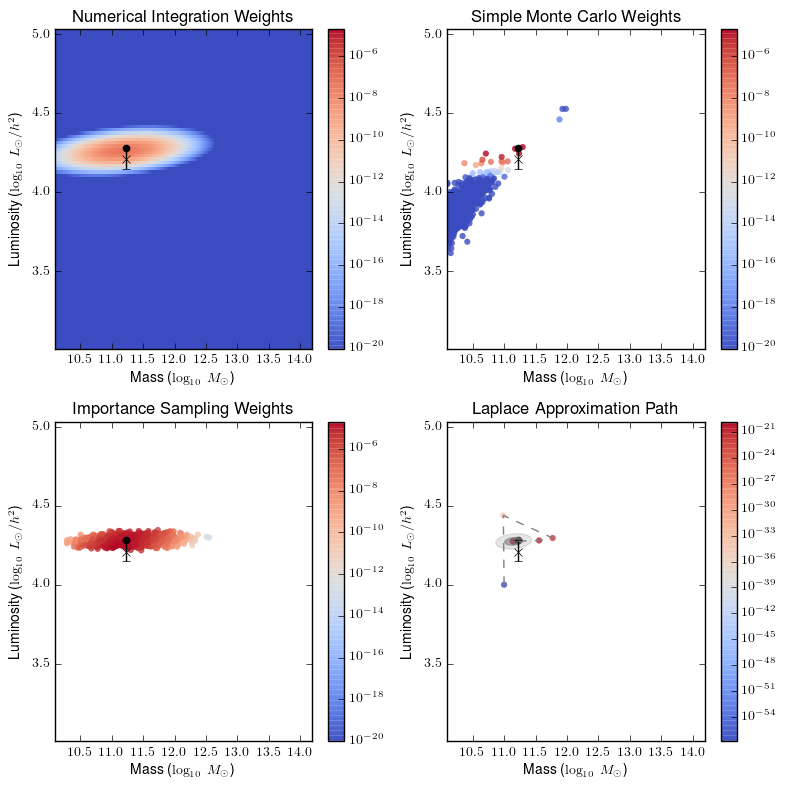
\includegraphics[width=0.9\columnwidth]{point1.png}
\caption{
The sampling panel for Point 0. Below are the returned values by the various methods.\\
numerical integration: 6.40358058377e-06\\
simple monte carlo: 8.57179497702e-07\\
importance sampling: 6.39959705909e-06\\
laplace approximation: 3.68701955823e-06\\
\label{fig:point1}}
\end{figure}

\begin{figure}[!h]
\centering
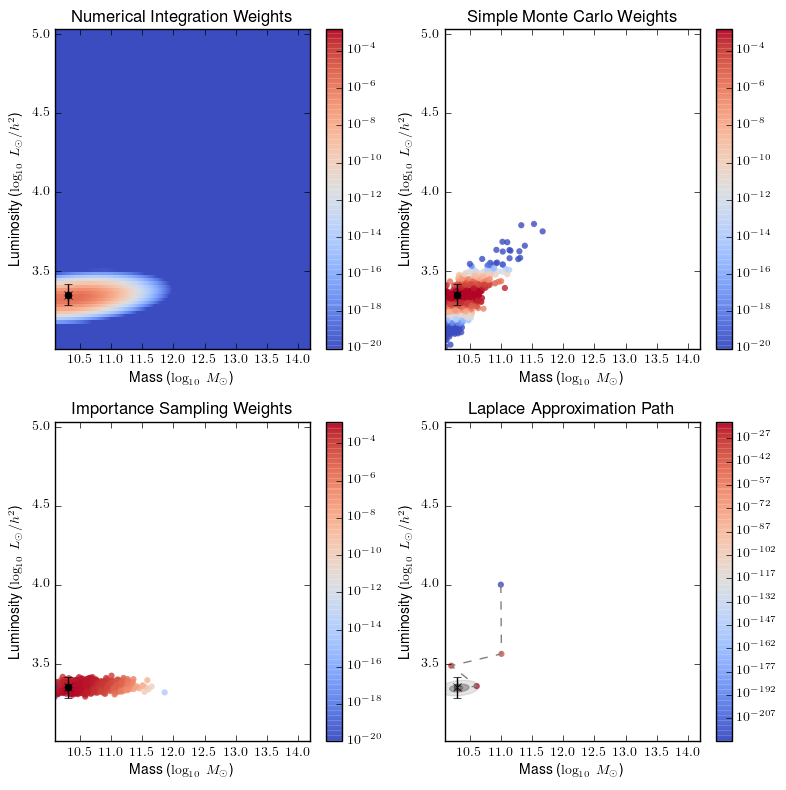
\includegraphics[width=0.9\columnwidth]{point2.png}
\caption{
The sampling panel for Point 1. Below are the returned values by the various methods.\\
numerical integration: 0.000487808661776\\
simple monte carlo: 0.000487547191603\\
importance sampling: 0.000487206370881\\
laplace approximation: 0.000316487709918\\
\label{fig:point2}}
\end{figure}

\begin{figure}[!h]
\centering
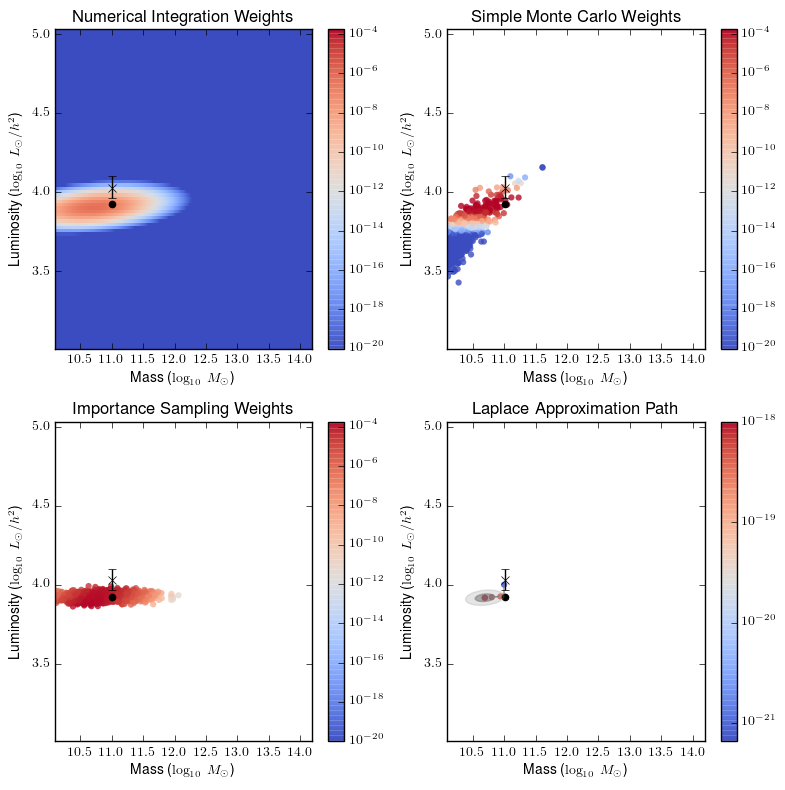
\includegraphics[width=0.9\columnwidth]{point3.png}
\caption{
The sampling panel for Point 2. Below are the returned values by the various methods.\\
numerical integration: 6.27613065943e-05\\
simple monte carlo: 2.82394491619e-05\\
importance sampling: 6.29604927168e-05\\
laplace approximation: 3.80374065466e-05\\
\label{fig:point3}}
\end{figure}

\begin{figure}[!h]
\centering
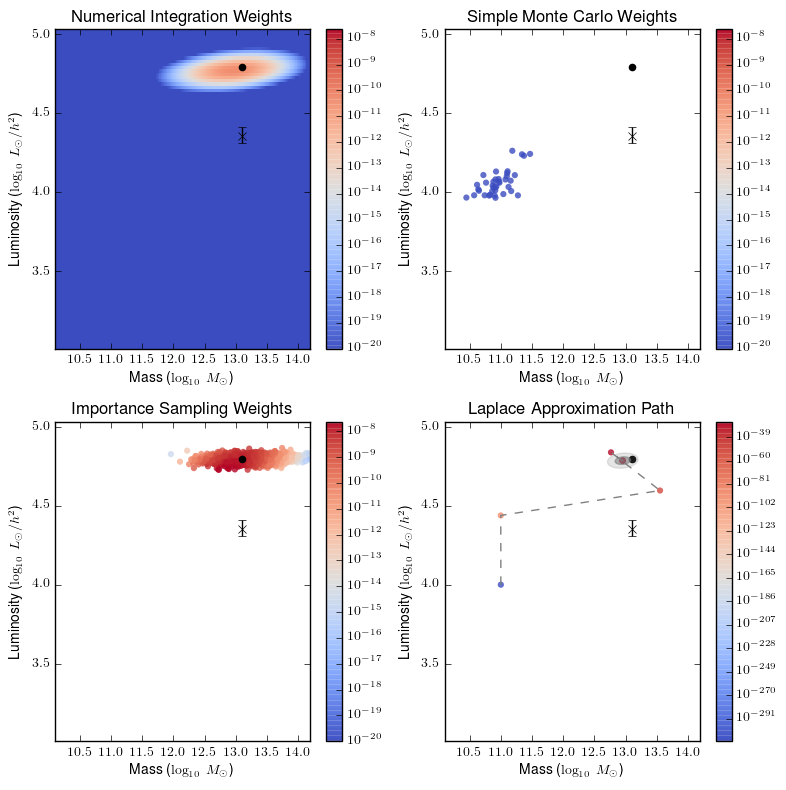
\includegraphics[width=0.9\columnwidth]{point4.png}
\caption{
The sampling panel for Point 3. Below are the returned values by the various methods.\\
numerical integration: 5.57536196939e-09\\
simple monte carlo: 3.49945536295e-53\\
importance sampling: 5.57880154767e-09\\
laplace approximation: 2.89024212204e-09\\
\label{fig:point4}}
\end{figure}

By sampling methodically over the entire region, numerical integration consistently computes the likelihood accurately.
Since the mass prior drops precipitously outside the displayed mass range, it is safe to assume that even for Point 1 (Figure \ref{fig:point2}) which appears cutoff, the technique still adequately covers the contributing region.
It serves as an answer key which we compare the other panels to. 

Simple monte carlo generates a narrow, diagonal slice of samples, which is consistent with the conditional luminosity relation.
Point 3 (Figure \ref{fig:point4}) shows how terribly suited this approach is for outlier halo likelihoods.
Even for Points 1 and 2 where it produces some high weight samples, it misses out on capturing the true oval shape of the high weight region.
While this approach has attractive computational aspects, its' inefficient sampling, fully exposed by outliers, renders it completely unsatisfactory.

Importance sampling is an attractive remedy to the problems that plague simple monte carlo.
Almost all the samples are high weight and the oval nature of the high weight region is captured.
Even in the outlier Point 3 (Figure \ref{fig:point4}), this technique performs very well.
The strong agreement between the solutions from this technique and numerical integration further reinforces our confidence.

The laplace approximation is a different approach entirely.
Here we see that the optimization finds the optimal point quickly, getting to within 0.1 distance within a handful of iterations.
But the hessian and the multivariate gaussian it produces seem a bit too small.
This visual intuition is confirmed by the consistent underestimating in the solutions.
The laplace approximation solutions are smaller than the solutions from numerical integration and importance sampling by a factor hovering around two.

Examining plots characterizing the sampling efficiency inspires many questions about the convergence and computational runtime of the different approaches. 
For convergence, we plot the returned value of the various methods for computing the halo likelihood for Point 0 under different numbers of samples (Figure \ref{fig:convergence}, top panel). 
Recall that samples in the context of numerical integration means luminosity samples, as the number of mass samples is fixed.
The laplace approximation does not use samples and is constant.
As expected, numerical integration and importance sampling converge to a stable value with fewer samples than simple monte carlo. 
Numerical integration and importance sampling require fewer samples than we had anticipated.
This pattern remains when we switch the likelihood to different halos. 

\begin{figure}[!h]
\centering
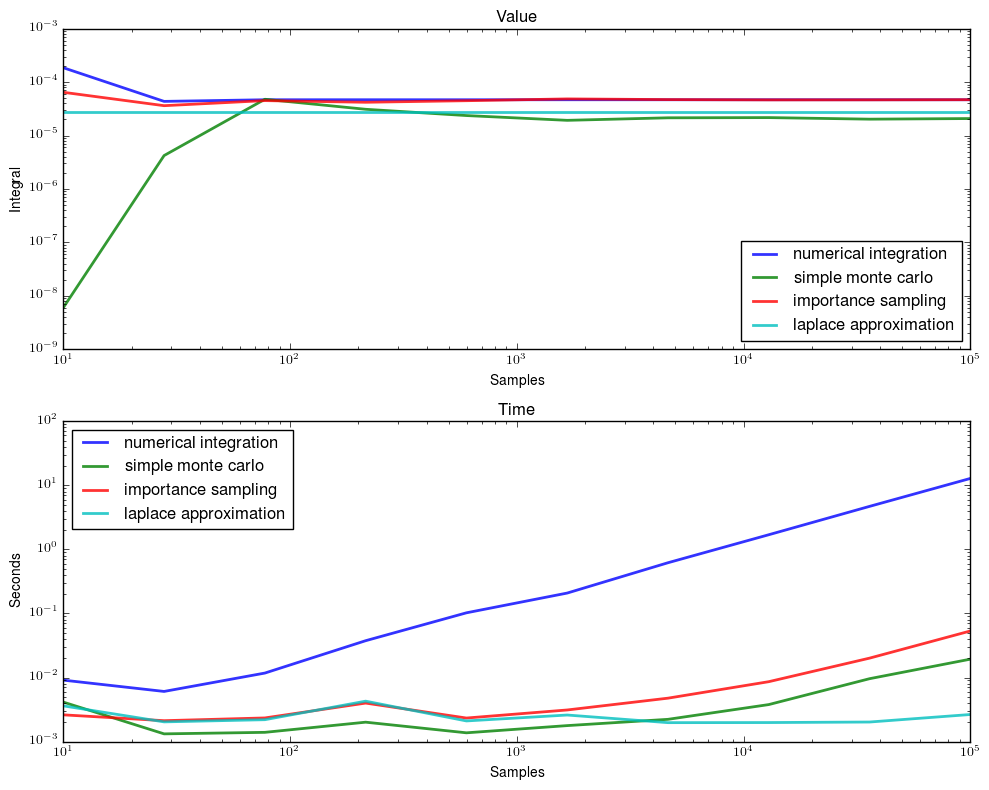
\includegraphics[width=0.9\columnwidth]{convergence.png}
\caption{
Top panel: the returned value of the likelihood integral for different numbers of samples.
Bottom panel: the runtime of the likelihood integral for different numbers of samples.
\label{fig:convergence}}
\end{figure}

Lowering the likelihood computation's runtime was the motivation for pursuing these alternative likelihood computations and remains an essential component of the analysis.
In the bottom panel of Figure \ref{fig:convergence} we show the runtime of the methods under different numbers of samples.
As before, the laplace approximation is constant (up to python interpreter and system jitter) because the number of samples is not a parameter.
As expected, the vast sampling numerical integration takes considerably longer than the other methods.
Importance sampling takes a little bit longer than simple monte carlo because of the four extra factors in the weight of each sample. 
At low number of samples the simple monte carlo and importance sampling methods are constant.
This is because the memory allocation in the sampling dominates the runtime.
Between $10^3-10^4$ samples, the vectorized computing begins to dominate and the relationship becomes linear. 

The highest level integration test we can do for the single halo likelihood situation is examine the resulting hyper-parameter likelihood surface. In Figure \ref{fig:posterior_all}, we fix all but one of the hyper-parameters which we do a line search over. 
We leave the hyper-parameter $\alpha_3$ out of this analysis because our prior for it is a delta function.
There is a large difference between the surface from laplace approximation and the other methods. Not only are some of the values and peaks far off, the curve itself is fairly jagged and erratic.
This makes us hesitant to employ it moving forward.

\begin{figure}[!h]
\centering
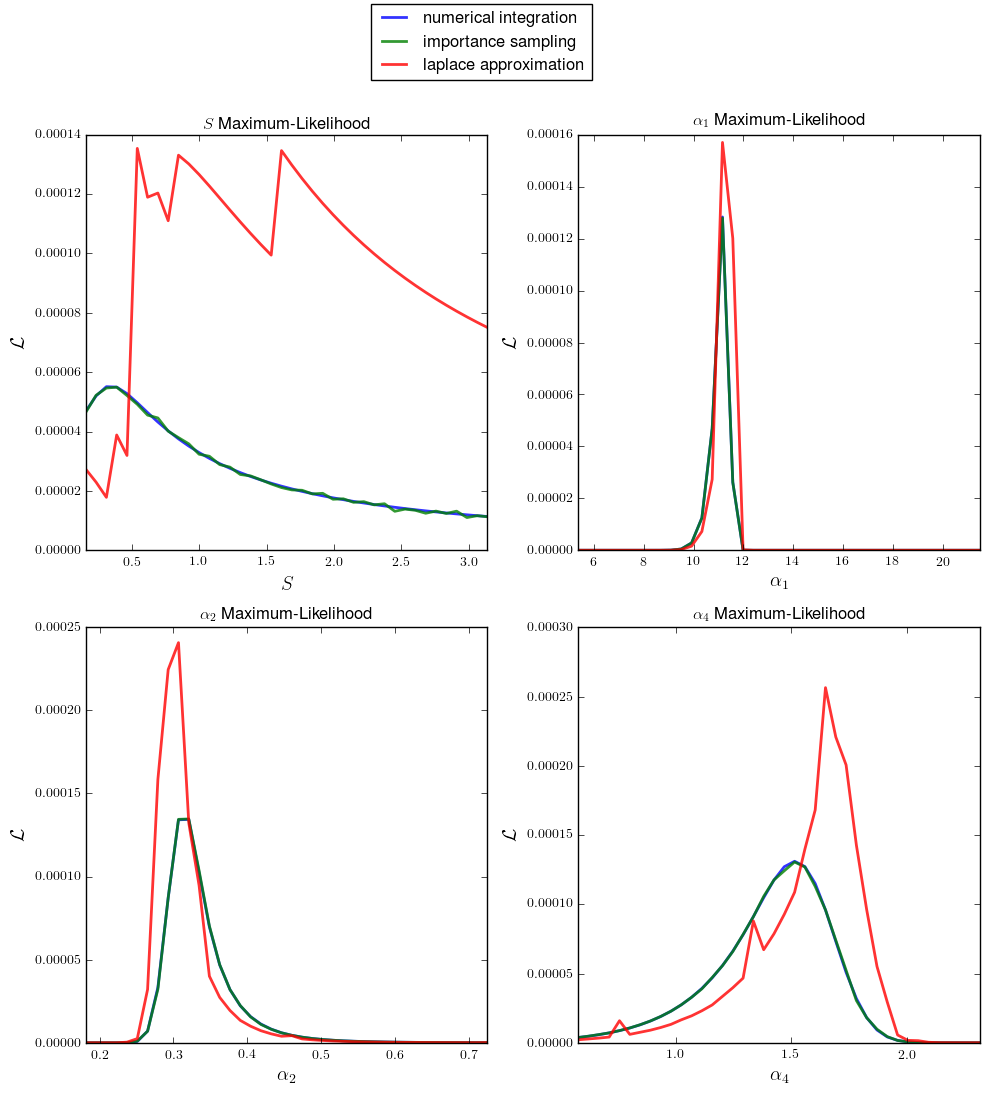
\includegraphics[width=0.9\columnwidth]{posterior_all.png}
\caption{
The single integral likelihood surfaces over lines in hyper-parameters $S, \alpha_1, \alpha_2, \alpha_4$. 
\label{fig:posterior_all}}
\end{figure}

The agreement between numerical integration and importance sampling is striking.
In Figure \ref{fig:posterior_is}, we narrow our focus to these two methods.
Here we generate an envelope of posterior values by running the importance sampling multiple times and allowing the inherent random sampling to take its course.
The posteriors are fairly smooth and even the 2$\sigma$ envelope tightly tracks the mean.

\begin{figure}[!h]
\centering
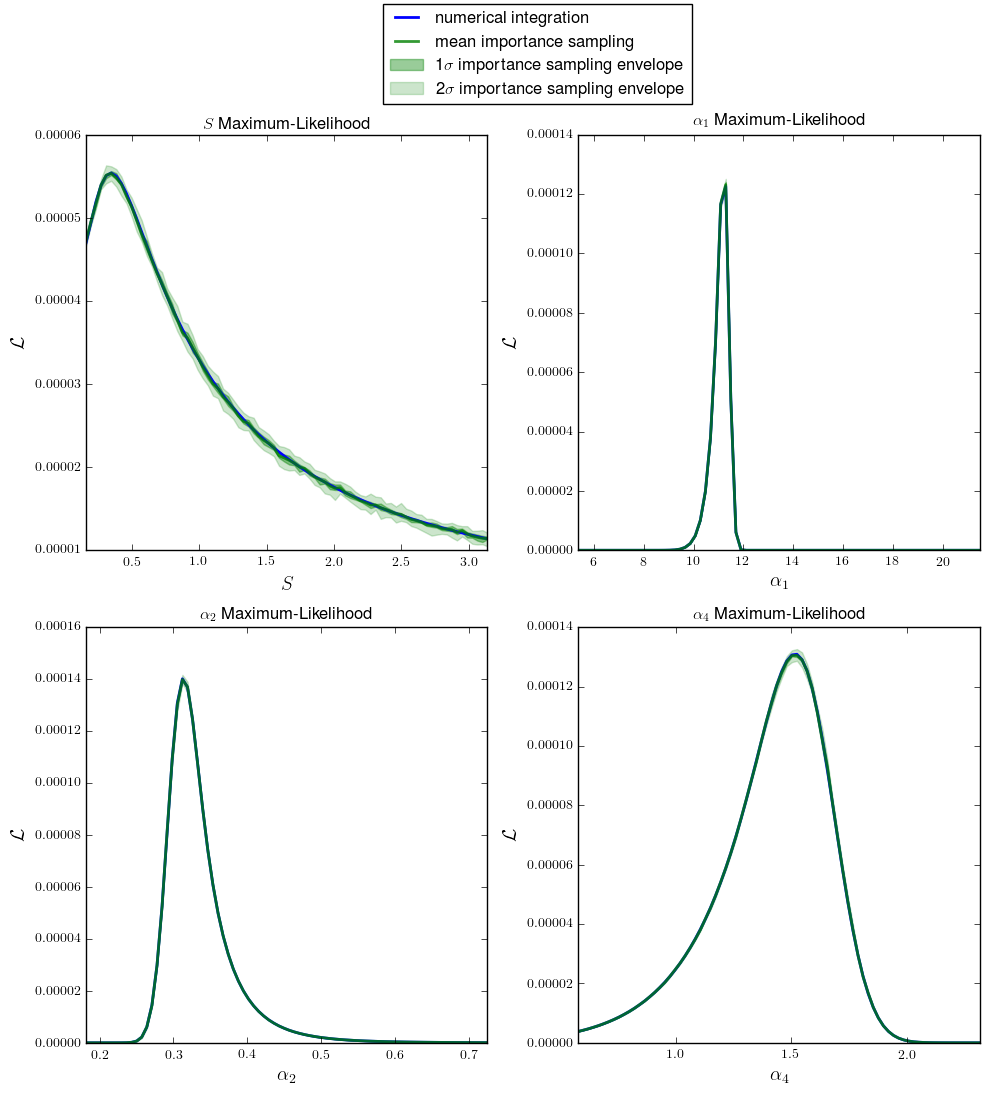
\includegraphics[width=0.9\columnwidth]{posterior_is.png}
\caption{
The single integral likelihood surfaces over lines in hyper-parameters $S, \alpha_1, \alpha_2, \alpha_4$.
We also include 1$\sigma$ and 2$\sigma$ envelopes of the importance sampling values, where the randomly drawn samples allow us to generate the distribution.
\label{fig:posterior_is}}
\end{figure}

\subsection{Scaling to Multiple Halos}

Now we shift from the characteristics of single halo likelihoods to the challenge of scaling these computations to multiple halos. 
The likelihood becomes a product of a large number of tiny integrals.
We switch to computing log likelihood because the tiny products break out of the bounds of the floating point exponent within a few products.
In Figure \ref{fig:scaling}, we measure the relationship between the number of likelihood halos (number of product integrals) and the runtime.
The simple linear relationship allows us to reliably extrapolate the runtime for the entire dataset.
Numerical integration over every halo in the dataset takes 15,593 seconds, or over 4 hours; importance sampling over every halo in the dataset takes 807 seconds, close to 10 minutes.
This is too long to expect wide adaption.
In Section \ref{sec:discussion} we discuss ways to further reduce the runtime.

\begin{figure}[!h]
\centering
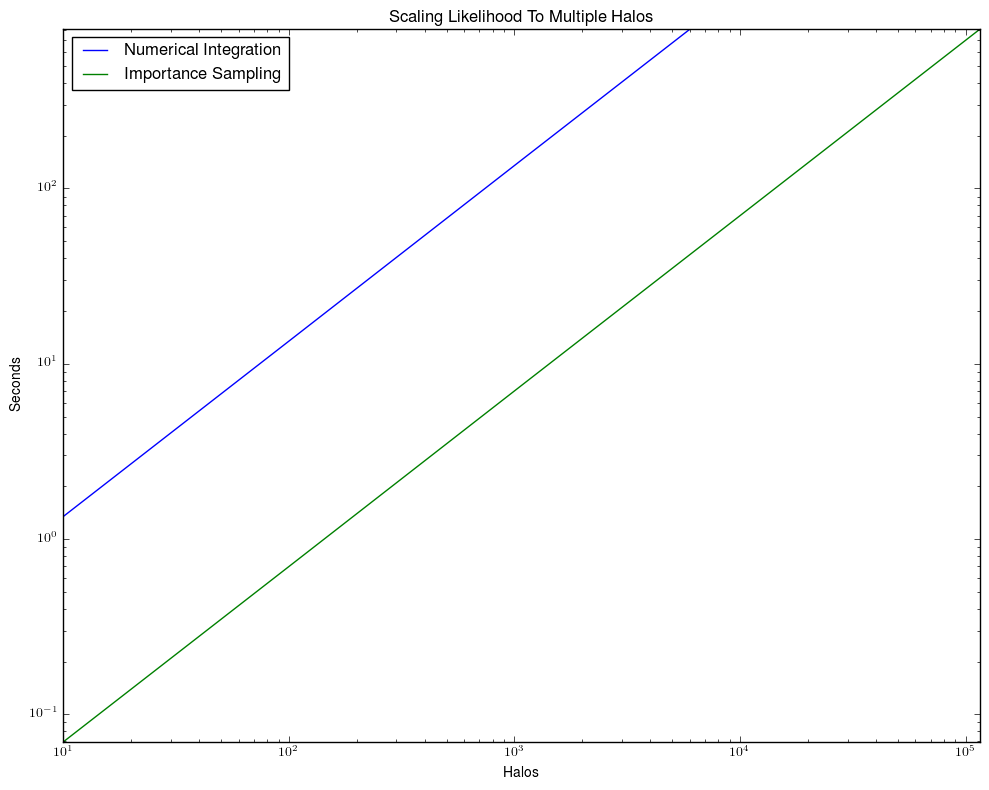
\includegraphics[width=0.9\columnwidth]{scaling.png}
\caption{
Scaling numerical integration and importance sampling to multiple halos.
\label{fig:scaling}}
\end{figure}

We also confirm that the maximum of the likelihood surface is near the hyper-parameters that generated the test dataset.
In Figure \ref{fig:multi_post}, we fix all but one of the hyper-parameters, which we do a line search over.
We use a randomly selected 100 halos from the dataset in the likelihood.
We leave the hyper-parameter $\alpha_3$ out of this analysis because our prior for it is a delta function.
The likelihood curves are smooth and have clearly distinguishable maxima.
These maxima are fairly close to the generating hyper-parameters, which is encouraging.
As we include more halos, we expect the maxima to grow closer to the generating hyper-parameters.

\begin{figure}[!h]
\centering
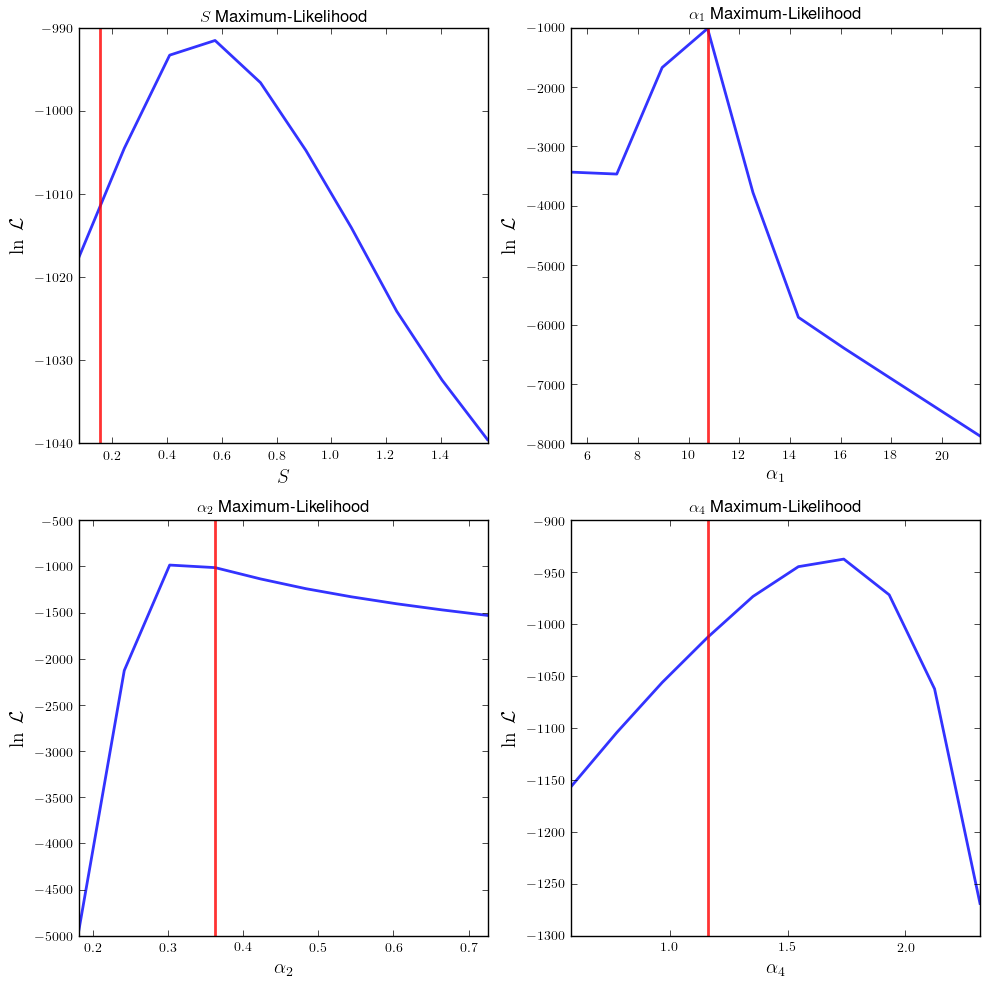
\includegraphics[width=0.9\columnwidth]{multi_post.png}
\caption{
The likelihood surfaces (in blue) for each of the nontrivial hyper-parameters along with the hyper-parameter value that generated the test dataset (in red). 
\label{fig:multi_post}}
\end{figure}

% ----------------------------------------------------------------------

\section{Discussion}
\label{sec:discussion}

\subsection{Interpretation of Single Integral Results}
\label{subsec:interp}
We have explored four methods for performing the likelihood corresponding to a single halo and marginalizing over masses and luminosities: numerical integration, simple monte carlo, importance sampling, and laplace approximation. [reiterate tradeoffs]

If we use a lognormal approximation in the laplace approximation we might better capture the tail of the distribution and produce more accurate approximations. We are interested in searching for a closed form solution of this problem in future work. 

Reproducibility is an essential feature of science. We encourage others to reproduce our results with the \emph{BigMaLI} python package which can be found on github at \code{https://github.com/davidthomas5412/BigMaLI}.

High performance computing is essential to our work. We have shaved off a lot of time on the importance sampling by implementing a fastlognorm method which outperforms \emph{scipy.stats.lognorm} sampling by a factor of 10. 

Another technology we explored is just in time compilation. For this we setup the \emph{numba} python package \citep{numba}. While there are lots of examples of numba accelerating pure python code, it struggles when modules that make calls to c/c++ are used. This is because the interpretter cannot collect runtime stats on these segments of the code. Our code makes heavy use of the \emph{numpy} module, so we measured an increase in runtime when using numba due to its overhead.

\subsection{Achieving Practical Runtime for Importance Sampling}
\label{subsec:achieve_runtime}

While implementing the likelihood codes we have simultaneously been regularly profiling our code. This makes us fairly confident that the current python implementation is about as fast as we can get from single process and thread python code. In importance sampling, each likelihood sample takes around 10 minutes. We expect that the markov chain monte carlo method we use to generate a posterior will require around 10,000 samples. With our current setup this would take seventy days.

Fortunately, we have many promising leads on how to further accelerate this computation. The first is reducing the number of mass and luminosity samples used in each integral. Figure \ref{fig:is_convergence} shows that we can still achieve decent accuracy with 1,000 samples per halo as opposed to our default of 10,000. This will reduce the runtime by a factor of one third.

\begin{figure}[h]
\centering
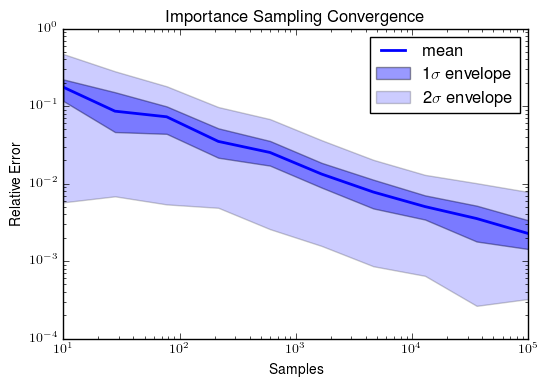
\includegraphics[width=0.9\columnwidth]{is_convergence.png}
\caption{
The accuracy of importance sampling against the number of mass and luminosity samples it consumes. The distribution for the 1$\sigma$ and 2$\sigma$ envelopes is generated from the random samples in different importance sampling runs.
\label{fig:is_convergence}}
\end{figure}

The major bottleneck with our python implementation is the sampling and evaluations where we heavily exploit numpy. Each time numpy methods are called the operating system must allocate new memory. We have implemented lognormal sampling code in python and c++ for comparison. We find that the c++ code, which efficiently reuses memory, is faster by a factor close to 15. By reimplementing our code in c++ we can achieve a 15x speedup and transition from being memory-allocation-bound to CPU-bound.

Finally, there are great computational resources available at the Stanford National Accelerator Laboratory. The Sherlock batch cluster has over 500 multicore nodes. The MCMC sampling can also be parallelized, increasing throughput close to linearly. Assuming that we can access 1,000 cores by using the Message Passing Interface (MPI), we expect to achieve close to a 1,000 times speedup of our posterior sampling.

Combining these speedups we find that we can achieve a throughput of 0.04 seconds per sample and complete the entire inference in 5 minutes.

% ----------------------------------------------------------------------

\section{Conclusions}
\label{sec:conclusions}

We have examined four different methods for computing the likelihood for our inference: numerical integration, simple monte carlo, and importance sampling. We find importance sampling to provide the best combination of accuracy and performance. Furthermore, we have a clear path from lowering the already accelerated likelihood runtime from approximately 10 minutes to 0.04 seconds.


% ----------------------------------------------------------------------

\subsection*{Acknowledgments}

% 
This is the text imported from \code{acknowledgments.tex}, and will be replaced by some standard LSST DESC boilerplate at some point.
% 


\input{contributions}

%{\it Facilities:} \facility{LSST}

% Include both collaboration papers and external citations:
\bibliography{main}

\newpage

\section{Appendix}
\label{sec:appendix}

\subsection{Epsilon Mass Function Background}
\label{subsec:epsilon_back}
Throughout the inference we use logarithms to improve numerical stability.
The \emph{log} function is not defined at zero which creates issues when sample halos are outside the bounds of the mass prior. 
A simple solution is adding a small background probability so that the function is always nonzero. 
There are two further modifications that must be made to make this work. 
First, the prior density must be recomputed so that it integrates to one.
Forgetting to do this leads to nontrivial accumulated errors in the importance sampling.
The second issue is when we sample from the prior we would not like many samples outside the original priors' support.
By making the background probability, which we call $\epsilon$, very small we can ensure that almost all samples are from the mass range of the original prior. 
We set $\epsilon = 10^{-30}$ over the mass range $[10^0, 100 * \text{MaxMass}]$ and renormalize the probability density accordingly.
In expectation, every $\sim 10^{30-18} = 10^{12}$ samples we draw lie outside the original support.
This small number will have negligible impact.
Figure \ref{fig:epsback} shows the updated mass function prior.

\begin{figure}[h]
\centering
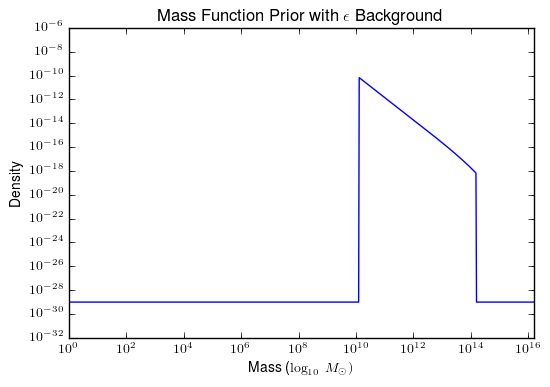
\includegraphics[width=0.6\columnwidth]{epsback.png}
\caption{
The mass function prior for z = 0 over the full range.
\label{fig:epsback}}
\end{figure}

\newpage

\subsection{Importance Sampling Is An Unbiased Estimator}
\label{subsec:is_unbiased}

We prove that in expectation, the mean attained from importance sampling is the true mean of the distribution.
Consider $\mu = \int_D dx\ f(x)p(x)$ where $D$ is the domain of integration, $f$ is the integrand, and $p$ is the probability density function on $D$. Then the chosen bias density function $q$, which is nonzero over $D$, can be used so that

$$\mu = E_p[f(x)] = \int_D dx\ f(x)p(x) = \int_D dx\ \frac{f(x)p(x)}{q(x)}q(x) = E_q\left[\frac{f(x)p(x)}{q(x)}\right]$$ 

\noindent This shows that the expected mean from importance sampling is the true mean of the distribution, as desired.
For readers who would like to learn more about this technique, we recommend perusing Chapter 9 in \citealt{mcbook}.

\newpage

\subsection{Converting Conditional Luminosity Scatter To Conditional Mass Scatter With Error Propagation}
\label{subsec:error_prop}

In Section \ref{subsec:is} we describe the biased distribution $Q(M|L, \alpha, S, z)$. 
Here we derive a conversion factor $\lambda$ such that $S_Q = \lambda \cdot S$ in the biased distribution. 
We use gaussian error propagation in log-space to approximate the log-variance in mass ($S_Q$) from the log-variance in luminosity ($S$).

\begin{align*}
S_Q^2 &= \left(\frac{\partial \ln \mu_M}{\partial \ln L}\right)^2 \cdot S^2\\
S_Q &= \left|\frac{\partial \ln \mu_M}{\partial \ln L}\right| \cdot S\\
\end{align*}

\noindent Plugging in the mean mass formula above and differentiating with respect to L yields

$$\frac{\partial \ln \mu_M}{\partial \ln L} = 1/\alpha_2$$

\noindent It is in our best interest to choose a conservative biased distribution so that if the center of the bias distribution is a little off the `important' region we can still get a few samples in the high weight region. In practice this means choosing a larger scatter. Therefore, we multiply the log-variance in luminosity by an extra factor of 2.

$$S_Q = \frac{2S}{\alpha_2}$$

\noindent We make a distribution of $S_Q$, shown in Figure \ref{fig:error_prop}, by sampling from the prior for $S$ and plugging it into the formula above. The result is similar to the value we arrived at from visual inspection of joint distributions. In our code we hardcode the $\lambda$ factor to be the mean of this distribution 5.6578015811698101.

\begin{figure}[h]
\centering
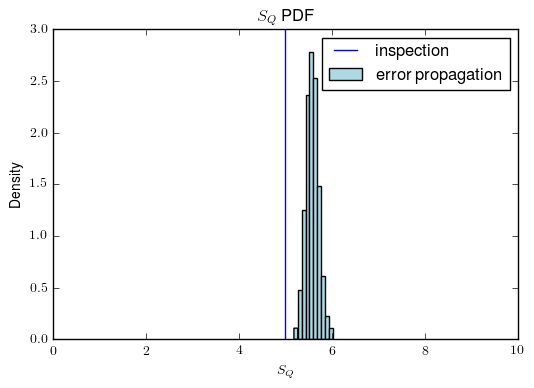
\includegraphics[width=0.6\columnwidth]{error_prop.png}
\caption{
The distribution of conversion factors from error propagation and the conversion factor from visual inspection of the data. 
\label{fig:error_prop}}
\end{figure}

\newpage

\subsection{Re-scaling The Laplace Approximation}
\label{subsec:rescale_la}

When implementing the laplace approximation as described in Subsection \ref{subsec:laplace}, we run into numerical issues.
The large difference in scale between masses and luminosities, differing by as much as $10^{10}$ at times, wipes out the precision in the off-diagonal terms of the Hessian matrix.
This manifests as having zeroes for the off-diagonal elements of the Hessian.
To avoid these issues we run the optimizer over the log mass and log luminosity.
In this section we describe the mathematics that makes this possible.
\\
\noindent Let f represent the log integrand, 

$$f(M,L) = \ln P(L^{obs}|L, \sigma_L^{obs}) + \ln P(L|M, \alpha, S, z) + \ln P(M|z)$$

\noindent Then we use the BFGS algorithm to attain

$$\ln M_{opt}, \ln L^{opt}, H_{ln}^{opt\ -1} = \text{argmin}_{\ln M,\ln L} -\left[f(M,L)\right]$$

\noindent where we optimize over logarithmic mass and luminosity to get an accurate hessian. Then by the chain rule we have 

$$-\frac{\partial^2 f}{\partial M \partial L} = -\frac{\partial^2 f}{\partial \ln M \partial \ln L} \frac{\partial \ln M}{\partial M} \frac{\partial \ln L}{\partial L} = -\frac{1}{ML}\frac{\partial^2 f}{\partial \ln M \partial \ln L}$$

\noindent After extending this to the other combinations of mass and luminosity we have

$$H^{opt} = (H_{ln}}^{opt\ -1})^{-1} \odot \begin{pmatrix}M^{opt}^{-2} & M^{opt}^{-1}L^{opt}^{-1}\\ M^{opt}^{-1}L^{opt}^{-1} & L^{opt}^{-2} \end{pmatrix}$$

\noindent where $\odot$ is elementwise multiplication. Then we can approximate the likelihood as 

$$\mathcal{L}(L^{obs}|\alpha, S, \sigma_L^{obs}, z) = \exp(f(M^{opt}, L^{opt}))\sqrt{\frac{(2\pi)^2}{\det(H^{opt})}}$$

\noindent Now the optimizer provides a Hessian with nonzero off-diagonal entries which produces a much better approximation.


\end{document}
% ======================================================================
% 
